% SYPT -- Unified salt-ice-water model, with the can (second edition)
% Built by .github/workflows/b8-report.yml with pdfLaTeX; standard packages only.
% Compile by hand: pdflatex sypt_salt_ice_model.tex (three times, for the contents and references).
\documentclass[11pt,a4paper]{article}

\usepackage[T1]{fontenc}
\usepackage[utf8]{inputenc}
\usepackage{lmodern}
\usepackage[margin=2.3cm,headheight=14pt]{geometry}
\usepackage{amsmath,amssymb,mathtools}
\usepackage{booktabs,tabularx,array,longtable}
\usepackage{xcolor}
\definecolor{accentA}{HTML}{1F5FA8}
\definecolor{accentB}{HTML}{C2410C}
\definecolor{corr}{HTML}{B91C1C}
\usepackage[most]{tcolorbox}
\usepackage{enumitem}
\usepackage{tikz}
\usepackage{fancyhdr}
\usepackage{microtype}
\usepackage[colorlinks=true,linkcolor=accentA,urlcolor=accentA,citecolor=accentA]{hyperref}

\newtcolorbox{worked}[1]{enhanced,breakable,colback=black!3,colframe=black!25,boxrule=0.5pt,arc=2pt,
  left=6pt,right=6pt,top=3pt,bottom=3pt,fonttitle=\bfseries\small,coltitle=black,
  title={Worked example: #1}}
\newtcolorbox{correction}{enhanced,breakable,colback=corr!4,colframe=corr!60,boxrule=0.6pt,arc=2pt,
  left=6pt,right=6pt,top=3pt,bottom=3pt}

\newcommand{\dd}{\mathrm{d}}
\newcommand{\dC}{\,{}^{\circ}\mathrm{C}}
\newcommand{\Troom}{T_{\mathrm{room}}}
\newcommand{\Ceff}{C_{\mathrm{eff}}}
\newcommand{\Cdeff}{C_{d,\mathrm{eff}}}
\newcommand{\Csat}{C_{\mathrm{sat}}}
\newcommand{\Hsol}{\Delta H_{\mathrm{sol}}}
\newcommand{\MN}{M_{\mathrm{NaCl}}}
\newcommand{\Aseg}{A_{\mathrm{seg}}}
\newcommand{\hov}{h_{\mathrm{ov}}}
\newcommand{\Tfd}{T_{fd}}
\newcommand{\Tabs}{\mathcal{T}}
\newcommand{\para}[1]{\par\smallskip\noindent\textbf{#1}\enspace}

\pagestyle{fancy}
\fancyhf{}
\lhead{\small SYPT: salt--ice--water modelling}
\rhead{\small Equation compendium, with the can}
\cfoot{\thepage}

\setlength{\parindent}{0pt}
\setlength{\parskip}{5pt}
\setlist{itemsep=2pt,topsep=4pt}

\title{\textbf{Unified Salt--Ice--Water Model, with the Can}\\[4pt]
  \large Full equation compendium and step-by-step derivations: second edition\\[3pt]
  \normalsize Styrofoam heat transfer, ice melting, NaCl dissolution, and a drink can\\
  that may be part-filled and may contain ethanol}
\author{SYPT modelling notes}
\date{29 October 2026}

\begin{document}
\maketitle

\begin{abstract}
This second edition expands every step of the first (26 October 2026) and adds the can of drink that the
bath is there to cool. Each equation is derived from the ones before it, line by line, with the
assumption it needs, a check, and a worked number. Steps~1--7 are the bath, as before: the first law, the
heat that leaks in through the Styrofoam, the ice, the water, the heat of dissolving salt, the freezing
point and the rate at which salt dissolves. Steps~8--10 are new: the drink and its can as a second body
that gives heat to the bath; a can that is not completely full, standing or lying, held under or floating;
and an ethanol model of the drink, which fixes its heat capacity and how cold it can get before it starts
to turn to slush. Steps~11 and~12 rebuild the time-dependent and equilibrium models with the can in them.
As in the first edition, equations that need qualification or correction are labelled; they should not be
used as exact identities.
\end{abstract}

\tableofcontents
\clearpage

% =====================================================================
\section*{What is new in this edition, and how to read it}
\addcontentsline{toc}{section}{What is new in this edition, and how to read it}

The first edition modelled the bath alone: ice, brine and salt in a Styrofoam box. A bath is only there to
cool something, so this edition adds the can and its drink, and expands every step.

\begin{itemize}
\item \textbf{The can} (Steps~8--10). The drink and its can are a second body, with its own temperature
  $T_d$, that gives heat to the bath through the can wall. Step~8 derives that heat flow. Step~9 works out
  which part of the wall passes it when the can is not full, stands or lies, is held under or floats.
  Step~10 models the drink as a solution of ethanol, sugar and carbon dioxide in water, which fixes its
  heat capacity and the temperature at which it starts to freeze.
\item \textbf{The coupled models} (Steps~11--12). The time-dependent model and the equilibrium of the first
  edition are rebuilt with the drink's heat in them, and solved for the rig.
\item \textbf{Every step expanded.} Each step says what it does and what it assumes, derives each equation
  from the one before, checks it, and works a number.
\item \textbf{New corrections}, labelled like those of the first edition: the Styrofoam's air films
  (Step~2); the salt's own heat capacity (Step~5); the error of the dilute freezing law in strong brine,
  and the temperature at which the model's bath stops cooling (Step~6); and starting temperatures other
  than $0\dC$ in the equilibrium (Step~12).
\end{itemize}

\textbf{How each step is laid out.} \textbf{The idea} says in words what the step does. \textbf{Assumptions}
lists what it takes for granted. \textbf{Derivation} goes line by line: every equation follows from the ones
before it, and the text says how. Key results are boxed. \textbf{Check} tests a result against its units or
a limiting case. A shaded box works a number. \textbf{Where it fails} says when not to use the result.

\textbf{Two sets of numbers.} The first edition illustrated its equations with a small demonstration
bath. A can needs a bath big enough to cool it, so the new steps use the rig of the B8 experiment with
Can~2. Both sets are in Table~\ref{tab:sets}; each worked example says which it uses.

\begin{table}[ht]
\centering\small
\caption{The two sets of numbers used in the worked examples.}
\label{tab:sets}
\begin{tabularx}{\linewidth}{@{}l >{\raggedright\arraybackslash}X >{\raggedright\arraybackslash}X@{}}
\toprule
 & Demonstration (first edition) & Rig, with Can~2 \\
\midrule
Box & $k = 0.033$\,W\,m$^{-1}$K$^{-1}$, $A = 0.05$\,m$^2$, $d = 0.02$\,m, so $H = 0.0825$\,W\,K$^{-1}$ &
  30\,mm of expanded polystyrene: $H \approx 0.46$\,W\,K$^{-1}$ for the foam alone \\
Room & $25\dC$ & $28\dC$ \\
Ice & 0.200\,kg at $0\dC$ & 4.0\,kg at $0\dC$ \\
Water & 0.100\,kg at $0\dC$ & 1.6\,kg at $4\dC$ \\
Salt & 0.050\,kg & 1.0\,kg at $28\dC$, grains 0.5\,mm across \\
Drink & --- & 330\,g at $28\dC$: a cola, or a 5\,\% beer (Step~10) \\
Can & --- & aluminium, 13\,g; diameter 6.6\,cm, height 11.66\,cm; headspace 1.2\,cm when upright \\
Films & --- & $h_i = 400$, $h_o = 270$\,W\,m$^{-2}$K$^{-1}$ upright; both $\times1.2$ lying (Step~8) \\
\bottomrule
\end{tabularx}
\end{table}

% =====================================================================
\section{System, notation and assumptions}\label{sec:system}

A closed Styrofoam box holds a container of ice, liquid water (brine, once salt dissolves), solid NaCl and
dissolved NaCl: the \emph{bath}. A sealed can of drink sits in the bath. The room, at $\Troom$, leaks heat
into the bath through the box. The drink, at $T_d$, gives heat to the bath through the can wall. The bath,
at $T$, absorbs both by warming, by melting ice and by dissolving salt.

Let $m_i(t)$, $m_w(t)$ and $m_s(t)$ be the masses of ice, liquid water and \emph{dissolved} NaCl (kg). Let
$m_{s,0}$ be the solid salt added at the start and $m_{s,d,0}$ any salt dissolved at the start. Then
$M_w = m_{i,0} + m_{w,0}$ is all the water and $S_0 = m_{s,0} + m_{s,d,0}$ all the salt. Temperatures in
sensible-heat terms are in $^\circ$C (a temperature difference is the same in K); absolute temperature
appears only in Step~6, written $\Tabs$.

\para{Assumptions about the bath.}
\begin{enumerate}[label=\textbf{B\arabic*}]
\item \textbf{One bath temperature.} One temperature $T$ describes the whole bath. With no stirrer this
  is an idealisation: brine next to the can warms first (the B8 report models that spreading).
\item \textbf{Ice and brine in equilibrium.} Ice melts or freezes fast enough that, while both are present,
  the bath sits at the freezing point of its brine (Step~6).
\item \textbf{Salt dissolves at a finite rate} (Step~7), so the dissolved salt is a variable of its own.
\item \textbf{Constant properties.} Specific heats, the latent heat and the heat of solution are
  constants. The brine's heat capacity is that of its water.
\item \textbf{The box is a steady conductor} (Step~2): it stores no heat and passes heat in proportion to
  the temperature difference.
\item \textbf{Closed and still.} The lid is on, nothing evaporates, nothing is added during a run, and
  nothing does work on the bath.
\end{enumerate}

\para{Assumptions about the can and drink.}
\begin{enumerate}[label=\textbf{C\arabic*}]
\item \textbf{One drink temperature} $T_d$: free convection keeps the drink mixed (Step~8).
\item \textbf{Steady wall and films}: the can's wall and the liquid films on it store no heat.
\item \textbf{A sealed can}: the drink's mass is fixed, and the gas in the headspace holds negligible heat.
\item \textbf{Heat passes only where the wall has drink inside and brine outside} (Step~9).
\item \textbf{The drink's properties follow from its composition} (Step~10).
\end{enumerate}

{\small
\begin{longtable}{>{$}l<{$} >{\raggedright\arraybackslash}p{7.6cm} >{\raggedright\arraybackslash}p{4.0cm}}
\caption{Notation. Numbers are the constants used throughout; the rest is set by the experiment.}
\label{tab:notation}\\
\toprule
\text{Symbol} & Meaning & Value or unit \\
\midrule
\endfirsthead
\toprule
\text{Symbol} & Meaning & Value or unit \\
\midrule
\endhead
\multicolumn{3}{@{}l}{\textit{The bath (first edition)}}\\
k & Styrofoam conductivity & W\,m$^{-1}$K$^{-1}$ \\
A,\ d & area and thickness of the insulating layer & m$^2$, m \\
H = kA/d & conductance of the box & W\,K$^{-1}$ \\
T,\ \Troom & bath and room temperatures & $^\circ$C \\
m_i,\ m_w,\ m_s & ice, liquid water, dissolved NaCl & kg \\
M_w,\ S_0 & all the water, all the salt & kg \\
W = M_w - m_i & liquid water, equal to $m_w$ & kg \\
c_i,\ c_w & specific heats of ice and liquid water & 2100, 4180\,J\,kg$^{-1}$K$^{-1}$ \\
c_s & specific heat of solid NaCl & 864\,J\,kg$^{-1}$K$^{-1}$ \\
L_f & latent heat of melting ice at $0\dC$ & 333\,500\,J\,kg$^{-1}$ \\
\MN & molar mass of NaCl & 0.05844\,kg\,mol$^{-1}$ \\
\Hsol & molar heat of solution of NaCl & 3900\,J\,mol$^{-1}$ \\
\beta = \Hsol/\MN & heat of solution per kg & 66\,735\,J\,kg$^{-1}$ \\
K_f & cryoscopic constant of water & 1.86\,K\,kg\,mol$^{-1}$ \\
i_v & van 't Hoff factor: ions per formula unit (named $i_v$ to avoid the ice index) & 2 \\
\alpha = i_vK_f/\MN & freezing-point coefficient & 63.65\,K \\
b & molality: moles of solute per kg of liquid water & mol\,kg$^{-1}$ \\
k_m & dissolution mass-transfer coefficient & m\,s$^{-1}$ \\
A_s & exposed surface area of the salt crystals & m$^2$ \\
C,\ \Csat & salt per volume of water; the same at saturation & kg\,m$^{-3}$; $\Csat \approx 357$ \\
\rho_w & density of water & 1000\,kg\,m$^{-3}$ \\
\Ceff = m_ic_i + Wc_w & heat capacity of the ice and water & J\,K$^{-1}$ \\[3pt]
\multicolumn{3}{@{}l}{\textit{The can and drink (new)}}\\
T_d & drink temperature & $^\circ$C \\
m_d,\ c_d & drink mass; drink specific heat (Step~10) & kg; J\,kg$^{-1}$K$^{-1}$ \\
m_c,\ c_c & can mass; specific heat of aluminium & kg; 900\,J\,kg$^{-1}$K$^{-1}$ \\
C_d = m_dc_d + m_cc_c & heat capacity of the drink and can & J\,K$^{-1}$ \\
r,\ \ell & radius and height of the can & m \\
t_w,\ k_w & wall thickness; conductivity of can aluminium & m; 160\,W\,m$^{-1}$K$^{-1}$ \\
h_i,\ h_o & drink-side and brine-side film coefficients & W\,m$^{-2}$K$^{-1}$ \\
\hov & overall coefficient through both films and the wall & W\,m$^{-2}$K$^{-1}$ \\
A_c & area of wall with drink inside and brine outside & m$^2$ \\
G = \hov A_c & conductance from the drink to the bath & W\,K$^{-1}$ \\
\dot Q_d = G(T_d - T) & heat flow from the drink to the bath & W \\
h_g & headspace height, can upright & m \\
f & fill fraction: share of the can's volume that is drink & --- \\
z_d,\ z_b & upright can: drink height; depth of brine on the can & m \\
y_d,\ y_g,\ y_b & lying can: drink depth; gas-strip depth; depth of brine on the can & m \\
\Aseg(y),\ P(y) & area and arc length of a circular segment of depth $y$ & m$^2$, m \\
\rho_d,\ \rho_b & densities of the drink and of strong brine & kg\,m$^{-3}$; $\rho_b \approx 1182$ \\[3pt]
\multicolumn{3}{@{}l}{\textit{The drink as a solution (new)}}\\
\mathrm{ABV} & alcohol by volume & --- \\
w_e,\ w_{su},\ w_c,\ w_x & mass fractions of ethanol, sugar, CO$_2$ and other extract in the drink & --- \\
w_{wd},\ m_{wd} & mass fraction and mass of water in the drink & ---, kg \\
M_e,\ M_{su},\ M_{c} & molar masses: ethanol, sucrose, CO$_2$ & 0.04607, 0.3423, 0.04401\,kg\,mol$^{-1}$ \\
\rho_e & density of ethanol at $20\dC$ & 789.2\,kg\,m$^{-3}$ \\
\Tfd & temperature at which the drink starts to freeze & $^\circ$C \\
\psi & share of the drink's water that is frozen & --- \\
\Cdeff & effective heat capacity of a freezing drink & J\,K$^{-1}$ \\
\bottomrule
\end{longtable}}

% =====================================================================
\section{Step 1: energy in = energy out}\label{sec:s1}

\para{The idea.} Energy is not created or destroyed. Heat that enters the bath either stays in it, as a
change of its energy, or leaves again. The can adds a second body to keep account of.

\para{The first edition's framing.}
\begin{align}
E_{\mathrm{in}} &= E_{\mathrm{out}}, \label{eq:s1-balance}\\
E_{\mathrm{in}} - E_{\mathrm{out}} &= \Delta U, \qquad U_{\mathrm{initial}} = U_{\mathrm{final}}\ \text{ if insulated and no work.}
\label{eq:s1-dU}
\end{align}

\para{Derivation.} The first law of thermodynamics for a \emph{closed} system, one that no mass crosses,
says that its internal energy $U$ changes by the heat $Q$ that enters it minus the work $W_{\mathrm{by}}$ it
does on its surroundings: $\Delta U = Q - W_{\mathrm{by}}$. Writing the net heat as what comes in minus
what goes out, $Q = E_{\mathrm{in}} - E_{\mathrm{out}}$, and taking $W_{\mathrm{by}} = 0$ gives
\eqref{eq:s1-dU}.

Why the work is zero: the bath does no work except expanding against the atmosphere, and for liquids and
solids that is tiny. Melting 1\,kg of ice shrinks it by $1/917 - 1/1000 = 9.1\times10^{-5}$\,m$^3$; at
atmospheric pressure that is $p\,\Delta V \approx 9$\,J, against the 333\,500\,J the melting takes. So here
the internal energy $U$ and the enthalpy $H = U + pV$ change by the same amount, and either may be used.

\eqref{eq:s1-balance} is the special case $\Delta U = 0$. It holds only when nothing accumulates, for
example in a steady state. While the bath cools or melts, its energy changes, and \eqref{eq:s1-dU} is the
correct statement. Dividing by a short time $\Delta t$ and letting it shrink turns energies into rates:
\begin{equation}
\frac{\dd U}{\dd t} = \dot Q_{\mathrm{in}}, \label{eq:s1-rate}
\end{equation}
with $\dot Q_{\mathrm{in}}$ the net heat flow into the system, in watts.

\para{Two bodies (new).} With the can there are two closed systems. The bath B receives heat through the
box, $\dot Q_{\mathrm{box}}$, and from the drink, $\dot Q_d$; the drink and can D lose $\dot Q_d$. Applying
\eqref{eq:s1-rate} to each, and adding:
\begin{align}
\frac{\dd U_B}{\dd t} &= \dot Q_{\mathrm{box}} + \dot Q_d, \label{eq:s1-bath}\\
\frac{\dd U_D}{\dd t} &= -\dot Q_d, \label{eq:s1-drink}\\
\frac{\dd (U_B + U_D)}{\dd t} &= \dot Q_{\mathrm{box}}. \label{eq:s1-sum}
\end{align}
$\dot Q_d$ is counted positive from the drink to the bath, so it leaves one body and enters the other, and
it cancels in the sum: only the box lets energy into the pair.

\para{Check.} Every term is in watts. With a perfect box, $\dot Q_{\mathrm{box}} = 0$, \eqref{eq:s1-sum}
says $U_B + U_D$ stays constant: what the drink loses, the bath gains.

\para{Where it fails.} If mass crosses the boundary --- the lid is lifted to add ice, or water
evaporates --- the systems are open, and the energy that mass carries must be added. A stirrer would add
its work; there is none here.

% =====================================================================
\section{Step 2: heat entering through Styrofoam}\label{sec:s2}

\para{The idea.} Heat flows from the warm room to the cold bath through the foam. Foam conducts poorly, so
the flow is small, and it is proportional to the temperature difference.

\para{Assumptions.} The foam wall is thin compared with its width, so heat flows straight through it (one
dimension). The foam stores no heat, so the flow is steady (B5). Its conductivity $k$ is uniform. And, as
in the first edition, its faces are at $\Troom$ and $T$.

\para{Derivation.} Fourier's law says that heat flows down a temperature gradient in proportion to it.
Take a coordinate $x$ through the wall from the bath side ($x = 0$) to the room side ($x = d$); the heat
flux toward the bath is $q = k\,\dd T/\dd x$ (W\,m$^{-2}$). If the foam stores no heat, whatever enters a
slice of it leaves the other side, so $q$ is the same at every $x$. Then $\dd T/\dd x$ is constant, and the
temperature rises in a straight line from $T$ to $\Troom$:
\[
\frac{\dd T}{\dd x} = \frac{\Troom - T}{d}, \qquad q = \frac{k}{d}\,(\Troom - T).
\]
Over an area $A$ the heat flow is $qA$. Adding it up over time, naming the conductance, and using
\eqref{eq:s1-rate} for the bath alone:
\begin{align}
\dot Q_{\mathrm{Styrofoam}}(t) &= \frac{kA}{d}\,\big(\Troom - T(t)\big), \label{eq:s2-Q}\\
Q_{\mathrm{in}}(t) &= \int_0^t \frac{kA}{d}\,\big[\Troom - T(\tau)\big]\,\dd\tau, \label{eq:s2-Qint}\\
H &= \frac{kA}{d}, \label{eq:s2-H}\\
\frac{\dd U}{\dd t} &= H\,\big(\Troom - T(t)\big). \label{eq:s2-dU}
\end{align}
$H$, in W\,K$^{-1}$, is the heat flow for each kelvin of difference. Walls, base and lid of different
thickness $d_j$ and area $A_j$ are separate paths side by side, so their flows add:
\begin{equation}
\dot Q_{\mathrm{in}} = \sum_j \frac{k_jA_j}{d_j}\,(\Troom - T). \label{eq:s2-sum}
\end{equation}

\para{Air films (correction).} The foam's faces are not at $\Troom$ and $T$: still air on each side adds a
film resistance $1/(hA)$ in series with the foam's $d/(kA)$. Resistances in series add, because the
temperature drops add while the heat flow is the same through each:
\begin{equation}
\frac{1}{H_j} = \frac{1}{h_{\mathrm{out}}A_j} + \frac{d_j}{k_jA_j} + \frac{1}{h_{\mathrm{in}}A_j}. \label{eq:s2-films}
\end{equation}
Still room air gives $h_{\mathrm{out}} \approx 9$\,W\,m$^{-2}$K$^{-1}$ (about 5 by convection and 4 by
radiation), and the air gap inside the box about 6. For 2\,cm of foam with $k = 0.033$, $d/k = 0.61$\,m$^2$K\,W$^{-1}$
while the films add $1/9 + 1/6 = 0.28$: the films cut the leak by about 30\,\%, and by 25\,\% for the rig's
3\,cm.

\para{Is the foam steady?} A temperature change crosses a layer of thickness $d$ in a time of order
$d^2/\kappa_f$, where $\kappa_f = k/(\rho_fc_f)$ is the foam's thermal diffusivity. For expanded polystyrene,
$\kappa_f = 0.035/(20\times1300) = 1.35\times10^{-6}$\,m$^2$\,s$^{-1}$: 300\,s for 2\,cm, 670\,s for 3\,cm.
After the first ten minutes or so the foam is steady. Before that it is still giving up heat it held at
room temperature, which \eqref{eq:s2-Q} leaves out.

\begin{worked}{the leak}
Demonstration: $H = 0.033\times0.05/0.02 = 0.0825$\,W\,K$^{-1}$; with the bath at $-10\dC$ and the room at
$25\dC$, $\dot Q = 0.0825\times35 = 2.9$\,W. Rig: 30\,mm of foam gives about 0.46\,W\,K$^{-1}$ alone and about
0.34 with its films and the gaps round the lid; with the bath at $-21\dC$ and the room at $28\dC$, 17 to
23\,W.
\end{worked}

\para{Where it fails.} Corners conduct more than flat walls, gaps round the lid let heat bypass the foam,
and the foam's own heat matters early on. Measuring $H$ directly, with the box test of the B8 README, is
more reliable than computing it.

% =====================================================================
\section{Step 3: the ice and the latent heat}\label{sec:s3}

\para{The idea.} Heat reaching the bath either warms what is there (sensible heat) or melts ice at constant
temperature (latent heat).

\para{Derivation.} The specific heat $c$ is the heat that warms 1\,kg by 1\,K, so warming a mass $m_i$ of
ice by $\dd T$ takes $m_ic_i\,\dd T$; dividing by $\dd t$ gives the rate. The latent heat $L_f$ is the heat
that melts 1\,kg of ice without changing its temperature, so melting $\dd m_{\mathrm{melt}}$ takes
$L_f\,\dd m_{\mathrm{melt}}$. Ice that melts is ice lost, $\dot m_{\mathrm{melt}} = -\dot m_i$:
\begin{align}
\dd Q_i &= m_ic_i\,\dd T, \label{eq:s3-dQi}\\
\dot Q_{i,\mathrm{sensible}} &= m_ic_i\,\dot T, \label{eq:s3-Qi}\\
\dd Q_{\mathrm{melt}} &= L_f\,\dd m_{\mathrm{melt}}, \label{eq:s3-dQm}\\
\dot Q_{\mathrm{melt}} &= L_f\,\dot m_{\mathrm{melt}}, \label{eq:s3-Qm}\\
\dot m_{\mathrm{melt}} &= -\dot m_i, \label{eq:s3-mm}\\
\dot Q_{\mathrm{melt}} &= -L_f\,\dot m_i. \label{eq:s3-Qm2}
\end{align}
The heat entering through the box warms the ice, warms the liquid water ($m_wc_w\dot T$, by the same
reasoning) and melts ice. Adding the three gives the first edition's combined balance:
\begin{equation}
H(\Troom - T) = (m_ic_i + m_wc_w)\,\dot T - L_f\,\dot m_i . \label{eq:s3-balance}
\end{equation}
When ice melts, $\dot m_i < 0$, so $-L_f\dot m_i$ is positive: melting absorbs heat.

\para{Check.} Pure ice and water coexist only at $0\dC$, so there $\dot T = 0$ and \eqref{eq:s3-balance}
gives $\dot m_i = -H(\Troom - T)/L_f$. Demonstration: $0.0825\times25/333\,500 = 6.2\times10^{-6}$\,kg\,s$^{-1}$,
22\,g of ice an hour.

\para{Where it fails.} $L_f$ is the latent heat at $0\dC$. Ice melting at $-15\dC$ takes less, by
$c_w - c_i$ for each kelvin below zero (Section~\ref{sec:refine}). Ice straight from a freezer at $-18\dC$
must first be warmed: $2100\times18 = 37.8$\,kJ\,kg$^{-1}$, 11\,\% of $L_f$.

% =====================================================================
\section{Step 4: liquid water and mass conservation}\label{sec:s4}

\para{The idea.} Water only changes form, ice to liquid or back, so ice and liquid always add up to the same
total.

\para{Derivation.} The liquid's sensible heat follows exactly as the ice's:
\begin{align}
Q_w &= m_wc_w\,\Delta T, \label{eq:s4-Qw}\\
\dot Q_{w,\mathrm{sensible}} &= m_wc_w\,\dot T . \label{eq:s4-Qwdot}
\end{align}
If melting and freezing are the only changes of form, and no water enters or leaves (B6), every kilogram of
ice lost is a kilogram of liquid gained. Integrating that from the start:
\begin{align}
\dd m_w &= -\dd m_i, \label{eq:s4-dm}\\
\dot m_w &= -\dot m_i, \label{eq:s4-mdot}\\
m_w(t) + m_i(t) &= m_{w,0} + m_{i,0} = M_w, \label{eq:s4-total}\\
m_w(t) &= M_w - m_i(t). \label{eq:s4-mw}
\end{align}
Substituting \eqref{eq:s4-mw} into \eqref{eq:s3-balance} leaves the ice as the only mass:
\begin{equation}
H(\Troom - T) = \big[m_ic_i + (M_w - m_i)\,c_w\big]\,\dot T - L_f\,\dot m_i . \label{eq:s4-balance}
\end{equation}

\para{Where it fails.} Dissolved salt makes the liquid heavier than its water but is given no heat
capacity here (B4): the brine's heat capacity is taken as that of its water.

% =====================================================================
\section{Step 5: enthalpy of dissolution of NaCl}\label{sec:s5}

\para{The idea.} Dissolving salt takes heat: pulling the crystal apart costs more energy than the water
molecules give back by gathering round the ions. A bath cools itself a little by dissolving its salt.

\para{Derivation.} A mass $m_s$ of dissolved salt is $n_s = m_s/\MN$ moles. The heat of solution $\Hsol$ is
measured per mole, so dissolving at a rate $\dot n_s$ absorbs $\Hsol\,\dot n_s$:
\begin{align}
n_s &= \frac{m_s}{\MN}, \label{eq:s5-ns}\\
\dot Q_{\mathrm{sol}} &= \Hsol\,\dot n_s = \frac{\Hsol}{\MN}\,\dot m_s = \beta\,\dot m_s, \label{eq:s5-Qsol}\\
\beta &= \frac{3900}{0.05844} = 66\,735\ \text{J\,kg}^{-1}. \notag
\end{align}
Dissolving is endothermic, $\beta > 0$: a positive $\dot m_s$ takes heat, so it joins the other heat sinks
on the right of \eqref{eq:s3-balance}:
\begin{equation}
\boxed{\,H(\Troom - T) = (m_ic_i + m_wc_w)\,\dot T - L_f\,\dot m_i + \frac{\Hsol}{\MN}\,\dot m_s\,} \label{eq:s5-balance}
\end{equation}
or, eliminating $m_w$ with \eqref{eq:s4-mw},
\begin{equation}
H(\Troom - T) = \big[m_ic_i + (M_w - m_i)\,c_w\big]\,\dot T - L_f\,\dot m_i + \beta\,\dot m_s . \label{eq:s5-balance2}
\end{equation}

\begin{worked}{dissolving}
Dissolving 1\,kg of salt absorbs 66.7\,kJ, as much as melting 0.20\,kg of ice. The demonstration's 50\,g
absorbs 3.3\,kJ, the heat of melting 10\,g of ice.
\end{worked}

\para{The salt's own heat capacity (correction).} Undissolved salt also warms and cools with the bath, at
$c_s = 864$\,J\,kg$^{-1}$K$^{-1}$, and \eqref{eq:s5-balance} leaves it out. To include it, add
$(S_0 - m_s)\,c_s$ to the heat capacity in front of $\dot T$. For the rig, 1\,kg of salt adds 864\,J\,K$^{-1}$
to the 15\,kJ\,K$^{-1}$ of its ice and water: 6\,\%. Steps~6--11 follow the first edition and leave it out;
the equilibrium of Step~12 includes it, with the heat the salt brings in from the room.

\para{Where it fails.} $\Hsol$ is measured in dilute solution at $25\dC$, and it changes with concentration
and temperature: one number is an approximation.

% =====================================================================
\section{\texorpdfstring{Step 6: freezing-point depression $i_vK_fb$}{Step 6: freezing-point depression}}\label{sec:s6}

\para{The idea.} Ice melts in brine below $0\dC$ because the dissolved ions dilute the water: ice and brine
can only coexist at a lower temperature than ice and pure water. While both are present the bath sits at
that temperature (B2), so the salt in the brine fixes the bath temperature.

\para{Where the law comes from.} Ice and liquid water exchange molecules until water has the same
\emph{chemical potential} --- Gibbs energy per mole --- in both. Ice is pure water. In the brine the ions
lower water's chemical potential below that of pure water, $\mu_w^*$, by $R\Tabs\ln a_w$, where $a_w < 1$ is
the water's activity, $R = 8.314$\,J\,mol$^{-1}$K$^{-1}$ and $\Tabs$ the absolute temperature:
\[
\mu_{\mathrm{ice}}(\Tabs) = \mu_w^*(\Tabs) + R\Tabs\ln a_w .
\]
At $\Tabs_0 = 273.15$\,K pure ice and water coexist. The Gibbs--Helmholtz relation, with the molar heat of
melting $\Delta h_{\mathrm{fus}} = L_fM_{\mathrm{H_2O}} = 333\,500\times0.018015 = 6008$\,J\,mol$^{-1}$,
turns the condition into
\[
\ln a_w = -\frac{\Delta h_{\mathrm{fus}}}{R}\Big(\frac{1}{\Tabs} - \frac{1}{\Tabs_0}\Big).
\]
In dilute brine, $\ln a_w$ is minus the moles of dissolved particles per mole of water. Each formula unit of
NaCl gives $i_v = 2$ ions, and $b$ moles of NaCl are dissolved in each kilogram of water, which is
$1/M_{\mathrm{H_2O}}$ moles of water, so $\ln a_w \approx -i_v\,b\,M_{\mathrm{H_2O}}$. For a small drop
$\Delta T_f = \Tabs_0 - \Tabs$, $1/\Tabs - 1/\Tabs_0 = \Delta T_f/(\Tabs\Tabs_0) \approx \Delta T_f/\Tabs_0^2$.
Equating the two expressions for $\ln a_w$:
\begin{gather}
\Delta T_f = \underbrace{\frac{R\Tabs_0^2M_{\mathrm{H_2O}}}{\Delta h_{\mathrm{fus}}}}_{K_f}\, i_v\, b , \label{eq:s6-Kf}\\
K_f = \frac{8.314\times273.15^2\times0.018015}{6008} = 1.86\ \text{K\,kg\,mol}^{-1}. \notag
\end{gather}
The ions are not quite independent: the osmotic coefficient, about 0.93 between 0.1 and 1\,mol\,kg$^{-1}$,
corrects for that, and in strong brine the logarithm can no longer be expanded.

\para{Derivation.} With $b$ in moles of NaCl per kilogram of \emph{liquid water}:
\begin{align}
\Delta T_f &= i_vK_fb, \label{eq:s6-dTf}\\
b(t) &= \frac{m_s(t)/\MN}{m_w(t)}, \label{eq:s6-b}\\
T_f(t) &= -i_vK_fb(t) = -\frac{i_vK_f\,m_s(t)}{\MN\,m_w(t)}, \label{eq:s6-Tf}\\
T(t) &= T_f(t)\quad\text{only when ice and brine coexist in equilibrium.} \label{eq:s6-coexist}
\end{align}
\eqref{eq:s6-b} is moles of salt over kilograms of water. \eqref{eq:s6-Tf} is the freezing point in
$^\circ$C, minus the drop. \eqref{eq:s6-coexist}: the bath sits at the freezing point only while there is
ice to melt or freeze. Substituting the mass balance \eqref{eq:s4-mw} and the shortcut
$\alpha = i_vK_f/\MN = 63.65$\,K:
\begin{equation}
\boxed{\,T = -\frac{i_vK_f\,m_s}{\MN\,(M_w - m_i)} = -\alpha\,\frac{m_s}{M_w - m_i}\,} \label{eq:s6-T}
\end{equation}
The bath gets colder as salt dissolves, and warmer as ice melts and dilutes the brine.

\begin{worked}{the first edition's example, and how accurate it is}
0.005\,kg of salt dissolved in 0.100\,kg of water:
\begin{equation}
T_f = -2\times1.86\times\frac{0.005/0.05844}{0.100} = -3.18\dC . \label{eq:s6-example}
\end{equation}
The measured freezing curve (Bodnar 1993) gives $-2.87\dC$ for this brine, 4.76\,wt\,\% salt: the dilute
law is 11\,\% too cold. In strong brine the error changes sign:

\smallskip
{\small\centering
\begin{tabular}{@{}lcccccc@{}}
\toprule
Salt in the brine (wt\,\%) & 5 & 10 & 15 & 16.5 & 20 & 23.2\\
\midrule
Dilute law, $\Delta T_f$ (K) & 3.35 & 7.07 & 11.23 & 12.58 & 15.91 & 19.21\\
Measured (Bodnar), $\Delta T_f$ (K) & 3.03 & 6.61 & 11.03 & 12.57 & 16.71 & 21.20\\
\bottomrule
\end{tabular}\par}
\end{worked}

\para{How much salt the brine can hold.} Brine holds at most $\Csat$ of salt; once it is saturated, extra
salt stays solid. With ice and saturated brine together, \eqref{eq:s6-T} with $m_s/W = \Csat/\rho_w$ gives
the coldest the model's bath can get:
\begin{equation}
T_{E,\mathrm{model}} = -\alpha\,\frac{\Csat}{\rho_w} . \label{eq:s6-TE}
\end{equation}
With halite's solubility, 357\,kg per m$^3$ of water (35.7\,g per 100\,g), this is $-22.7\dC$. The real
coldest point, the eutectic, is $-21.2\dC$ at 23.2\,wt\,\% (0.302\,kg of salt per kg of water), where the
dilute law gives $-19.2\dC$.

\begin{correction}
\textbf{Correction.} The dilute law \eqref{eq:s6-dTf} is good to about 10\,\% up to 15\,wt\,\%, but at the
eutectic composition it is 2\,K too warm, and with halite's solubility it puts the bath's floor at
$-22.7\dC$ instead of $-21.2\dC$. For strong brine, replace it with the measured freezing curve,
$W = 1.78\,\vartheta - 0.0442\,\vartheta^2 + 5.572\times10^{-4}\,\vartheta^3$ (wt\,\% of salt against
$\vartheta$ degrees below zero; Bodnar 1993), and the measured eutectic.
\end{correction}

% =====================================================================
\section{Step 7: salt dissolution rate and shrinking crystals}\label{sec:s7}

\para{The idea.} Salt dissolves from the surface of each grain. Right at the surface the brine is
saturated; further out it is weaker, and dissolved salt diffuses across the thin layer between. The rate is
the area of the grains times how fast salt crosses that layer.

\para{Derivation.} Fick's law: salt diffuses down its concentration gradient at a flux $D$ times the
gradient, with $D$ the diffusion coefficient. Across a layer of thickness $\delta$, from saturated brine at
the surface ($\Csat$) to the bulk ($C$), the flux is $D(\Csat - C)/\delta$ in kg\,m$^{-2}$s$^{-1}$. Calling
$k_m = D/\delta$ the mass-transfer coefficient and multiplying by the exposed area $A_s$:
\begin{align}
\dot m_s &= k_mA_s\,(\Csat - C), \label{eq:s7-rate}\\
C(t) &\approx \frac{\rho_w\,m_s(t)}{m_w(t)}, \label{eq:s7-C}\\
\dot m_s &\approx k_mA_s\Big[\Csat(T) - \frac{\rho_w m_s}{m_w}\Big]. \label{eq:s7-rate2}
\end{align}
\eqref{eq:s7-C} measures the concentration as salt per volume of water, $m_s/(m_w/\rho_w)$, close to salt
per volume of brine while the brine is dilute. For NaCl, $D \approx 1.5\times10^{-9}$\,m$^2$s$^{-1}$; a
layer 0.1\,mm thick, as when brine flows past the grains, gives $k_m \approx 10^{-5}$\,m\,s$^{-1}$, and a still
layer ten times thicker $10^{-6}$.

\para{Shrinking crystals.} Take $N$ grains of the same shape, each a cube of side $a$. Their mass is
$m_{\mathrm{solid}} = N\rho_{\mathrm{salt}}a^3$ and their area $6Na^2$. Eliminating $a$, the area is
$6N^{1/3}(m_{\mathrm{solid}}/\rho_{\mathrm{salt}})^{2/3}$: for a fixed number of similar grains it goes as the
solid mass to the power $\tfrac23$, whatever their shape. With no salt dissolved at the start:
\begin{align}
m_{\mathrm{solid}}(t) &= m_{s,0} - m_s(t), \label{eq:s7-solid}\\
A_s(t) &= A_{s,0}\Big(\frac{m_{s,0} - m_s(t)}{m_{s,0}}\Big)^{2/3}, \label{eq:s7-As}
\end{align}
so
\begin{equation}
\boxed{\,\dot m_s = k_mA_{s,0}\Big(\frac{m_{s,0} - m_s}{m_{s,0}}\Big)^{2/3}\Big[\Csat(T) - \frac{\rho_w m_s}{m_w}\Big]\,} \label{eq:s7-boxed}
\end{equation}

\begin{worked}{how fast the rig's salt dissolves}
1\,kg of grains 0.5\,mm across is $3.7\times10^6$ cubes, with $A_{s,0} = 5.5$\,m$^2$. In fresh water,
with $\Csat = 357$\,kg\,m$^{-3}$, the starting rate $k_mA_{s,0}\Csat$ is 20\,g\,s$^{-1}$ for
$k_m = 10^{-5}$\,m\,s$^{-1}$ (the lot in about a minute, were the rate to stay up) and 2\,g\,s$^{-1}$ for
$10^{-6}$ (about eight minutes). Both slow as the grains shrink and the brine strengthens.
\end{worked}

\para{Where it fails} (from the first edition). It needs $0 \le m_s < m_{s,0}$: undissolved salt must
remain, and the brine must be undersaturated. An extension that forbids precipitation uses
$\max(0, \Csat - C)$ and stops at complete dissolution. With salt dissolved at the start, use $S_0 - m_s$ in
place of $m_{s,0} - m_s$. For concentrated brine use $C = m_s/V_{\mathrm{brine}}$ with the measured brine
density. $k_m$ and $A_{s,0}$ depend on grain size, on how brine moves through the ice and on whether a crust
forms, and are best fitted to a run.

% =====================================================================
\section{Step 8: the can and its drink (new)}\label{sec:s8}

\para{The idea.} The drink and its can are a second body in the bath. It has one temperature $T_d$ and a
heat capacity $C_d$, and it gives heat to the bath through the can wall at a rate proportional to $T_d - T$.

\subsection{The drink as one body}
\para{Derivation.} Apply \eqref{eq:s1-drink} to the drink and can. With one temperature (C1) and constant
specific heats, their energy measured from a reference temperature is
$U_D = (m_dc_d + m_cc_c)(T_d - T_{\mathrm{ref}})$; the reference drops out on differentiating:
\begin{equation}
C_d\,\frac{\dd T_d}{\dd t} = -\dot Q_d, \qquad C_d = m_dc_d + m_cc_c. \label{eq:s8-drink}
\end{equation}
The gas in the headspace is left out (C3). A 41\,mL headspace of CO$_2$ at two atmospheres is
$pV/(R\Tabs) \approx 0.0035$\,mol, 0.15\,g, holding 0.13\,J\,K$^{-1}$: a ten-thousandth of $C_d$.

\begin{worked}{Can 2}
For a sugary soft drink, $C_d = 0.330\times4000 + 0.013\times900 = 1320 + 12 = 1332$\,J\,K$^{-1}$. The can
adds 1\,\%.
\end{worked}

\subsection{The heat path through the wall}
\para{Derivation.} Heat leaves the drink through three layers in series: the film of drink on the inside of
the wall, the aluminium, and the film of brine on the outside. By C2 none of them stores heat, so the same
heat flow crosses each, driven by the temperature drop across it. Per unit area a film passes $h\,\Delta T$
--- Newton's law of cooling, which defines the film coefficient $h$ --- and the wall $k_w\Delta T/t_w$, by
Fourier's law as in Step~2:
\[
\frac{\dot Q_d}{A_c} = h_i\,(T_d - T_{wi}) = \frac{k_w}{t_w}\,(T_{wi} - T_{wo}) = h_o\,(T_{wo} - T),
\]
with $T_{wi}$ and $T_{wo}$ the wall's inner and outer faces and $A_c$ the area that passes heat (Step~9).
Rearranging each to a temperature drop and adding them, the wall temperatures cancel:
\begin{equation}
\dot Q_d = G\,(T_d - T),\qquad G = \hov A_c,\qquad \frac{1}{\hov} = \frac{1}{h_i} + \frac{t_w}{k_w} + \frac{1}{h_o}. \label{eq:s8-G}
\end{equation}
The aluminium hardly matters: $t_w/k_w = 10^{-4}/160 = 6\times10^{-7}$\,m$^2$K\,W$^{-1}$, against
$1/h_i = 2.5\times10^{-3}$ and $1/h_o = 3.7\times10^{-3}$. A plastic sleeve label would add its own
resistance in series.

\subsection{The film coefficients}
\para{Derivation.} Nothing stirs the drink or the bath, so the films are set by free convection. Next to
the wall the liquid is $\Delta T$ warmer or colder than the rest, so lighter or denser by $\rho\beta_T\Delta T$,
with $\beta_T$ its thermal expansion coefficient, and buoyancy drives it along the wall. Balancing buoyancy
against viscosity, and the heat carried along the wall against the heat conducted across the layer, gives
a layer thickness $\delta_T \sim \mathcal L\,\mathrm{Ra}^{-1/4}$, where $\mathcal L$ is the height of the wall
and $\mathrm{Ra} = g\beta_T\Delta T\mathcal L^3/(\nu\kappa)$ the Rayleigh number ($\nu$ and $\kappa$ are the
liquid's viscosity and thermal diffusivity). The film coefficient is about $k/\delta_T$, so
\begin{equation}
h \propto \Big(\frac{\Delta T}{\mathcal L}\Big)^{1/4}. \label{eq:s8-h}
\end{equation}
The constant comes from experiments. This document takes $h_i = 400$ and $h_o = 270$\,W\,m$^{-2}$K$^{-1}$ for
an upright can at a 25\,K difference (a study of bottles, and a fit to a measured cooling time), and
multiplies both by 1.2 for a can lying on its side, whose relevant length is its 6.6\,cm diameter instead of
its 11.7\,cm height: $(11.66/6.6)^{1/4} = 1.15$ from \eqref{eq:s8-h} alone. Then $\hov = 161$ upright and
193 lying. In a part-filled upright can the drink's wall is only as tall as the drink, so $h_i$ is a few per
cent larger.

\subsection{Is one drink temperature enough?}
A still drink would not be uniform: its Biot number, $h_i(V/A)/k = 400\times0.0129/0.58 \approx 9$, is far
above the 0.1 below which conduction alone keeps a body uniform. It is uniform enough because free
convection stirs it: the cold layer on the wall is about 1\,mm thick and sinks, and the core is mixed. Cold
drink does collect at the bottom, so the core stratifies slowly; a probe at the top of the drink and one at
the bottom test C1.

\subsection{The fixed-bath solution}
\para{Derivation.} If the bath stays at $T$, \eqref{eq:s8-drink} with \eqref{eq:s8-G} is
$C_d\dot T_d = -G(T_d - T)$: the difference $T_d - T$ falls at a rate proportional to itself. Separating the
variables and integrating from $T_{d,0}$, then solving for the time to reach a target $T^*$:
\begin{equation}
T_d(t) = T + (T_{d,0} - T)\,e^{-t/\tau},\qquad \tau = \frac{C_d}{G},\qquad
t_{T^*} = \tau\ln\frac{T_{d,0} - T}{T^* - T}. \label{eq:s8-fixed}
\end{equation}

\begin{worked}{if the whole can passed heat}
The whole surface of Can~2 is $A_c = 2\pi r\ell + 2\pi r^2 = 242 + 68 = 310$\,cm$^2$. Upright, $G = 161\times0.0310
= 5.0$\,W\,K$^{-1}$ and $\tau = 1332/5.0 = 266$\,s; from $28\dC$ to $5\dC$ in a bath at $-18\dC$,
$t = 266\ln(46/23) = 185$\,s. Step~9 shows why less of the wall passes heat.
\end{worked}

\para{What it does to the bath.} The drink's heat enters the bath: $G(T_d - T)$ joins $H(\Troom - T)$ on
the left of the bath balance \eqref{eq:s5-balance} (Step~11).

% =====================================================================
\section{Step 9: a can that is not completely full (new)}\label{sec:s9}

\para{The idea.} A sealed can holds gas above its drink. Heat crosses the wall well only where there is
liquid on both sides: drink inside, brine outside. The gas also decides whether the can floats, and how much
room the drink has to expand if it freezes.

\subsection{What the headspace changes}
\begin{itemize}
\item \textbf{The drink's mass} is whatever is in the can: weigh it full and empty. The headspace does not
  change $C_d$ (Step~8).
\item \textbf{The wall with gas behind it passes almost no heat.} Heat would have to reach it through the
  gas, which conducts twenty to thirty times worse than water and barely convects in so thin a layer: a
  film coefficient of a few W\,m$^{-2}$K$^{-1}$, a hundred times less than $h_i$. So the area that passes
  heat, $A_c$, is the wall wetted by drink inside \emph{and} by brine outside (C4).
\item \textbf{Conduction along the aluminium} carries a little heat past the drink's surface. The wall acts
  as a fin whose reach is $\lambda = \sqrt{k_wt_w/h_o} = \sqrt{160\times10^{-4}/270} = 7.7$\,mm: a strip about
  that wide along the drink's surface passes some heat, adding up to about 6\,\% to $G$ for the upright
  can. It is left out, so the model slightly underestimates $G$.
\end{itemize}

\subsection{Measuring the fill}
Stand the can upright and measure the headspace height $h_g$, from the top of the cylinder to the drink's
surface; or fill an empty can with water to find its volume and subtract the drink's volume $m_d/\rho_d$.
Treating the can as a cylinder of radius $r$ and height $\ell$, the gas volume is $V_g = \pi r^2h_g$ and the
fill fraction $f = 1 - h_g/\ell$. A real can's neck and domed base hold less than $\pi r^2\ell$: Can~2's
cylinder would hold 399\,mL, against 330\,mL of drink and about 41\,mL of headspace. Measure volumes rather
than compute them.

\subsection{Upright can}
\para{Derivation.} The drink stands $z_d = \ell - h_g$ high. Inside, the side wall is wet up to $z_d$ and the
base all over; the lid has gas behind it. Outside, the brine reaches a depth $z_b$ up the can
($z_b \ge \ell$ when the can is held under). The wall is wet on both sides up to the lower of the two heights,
so the side wall passes heat up to that height, and the base passes heat everywhere:
\begin{equation}
A_c = 2\pi r\,\min(z_d, z_b) + \pi r^2 . \label{eq:s9-upright}
\end{equation}

\subsection{Lying can: the circular segment}
\para{Derivation.} Lying on its side, the can's cross-section is a circle of radius $r$, and the drink fills
the part below a horizontal chord: a circular \emph{segment}. A chord at height $y$ above the lowest point
is $r - y$ below the centre, so it subtends a half-angle $\theta$ at the centre with $\cos\theta = (r - y)/r$.
The segment is the sector of angle $2\theta$, of area $r^2\theta$, minus the triangle between the chord and the
centre, of area $(r - y)\,r\sin\theta = (r - y)\sqrt{2ry - y^2}$; and the arc below the chord is $2r\theta$
long:
\begin{gather}
\Aseg(y) = r^2\arccos\frac{r - y}{r} - (r - y)\sqrt{2ry - y^2}, \label{eq:s9-segment}\\
P(y) = 2r\arccos\frac{r - y}{r}. \notag
\end{gather}
The formula holds for $y > r$ too, where $r - y$ is negative and the ``triangle'' adds to the sector. Laying
the can down does not change the volume of its gas, so the gas strip along the top has the same volume as
the upright headspace. That fixes the strip's depth $y_g$, and the drink's depth is what is left:
\begin{equation}
\ell\,\Aseg(y_g) = \pi r^2h_g, \qquad y_d = 2r - y_g . \label{eq:s9-gas}
\end{equation}
With brine $y_b$ up the can, the wall is wet on both sides below $y = \min(y_d, y_b)$: along the length of
the can (the arc times $\ell$) and on the two flat ends (a segment each):
\begin{equation}
A_c = \ell\,P(y) + 2\,\Aseg(y),\qquad y = \min(y_d, y_b). \label{eq:s9-lying}
\end{equation}

\begin{worked}{Can 2 held under the brine}
$r = 3.3$\,cm, $\ell = 11.66$\,cm, $h_g = 1.2$\,cm. Upright: $z_d = 10.46$\,cm ($f = 0.897$) and
\eqref{eq:s9-upright} gives $A_c = 217 + 34 = 251$\,cm$^2$, 81\,\% of the whole surface. Lying:
\eqref{eq:s9-gas} needs a segment of $\pi r^2h_g/\ell = 3.52$\,cm$^2$, 10\,\% of the circle, so the gas strip is
$y_g = 1.05$\,cm deep and the drink $y_d = 5.55$\,cm; \eqref{eq:s9-lying} gives $A_c = 178.5 + 61.4 = 240$\,cm$^2$,
77\,\%.
\end{worked}

\begin{figure}[ht]
\centering
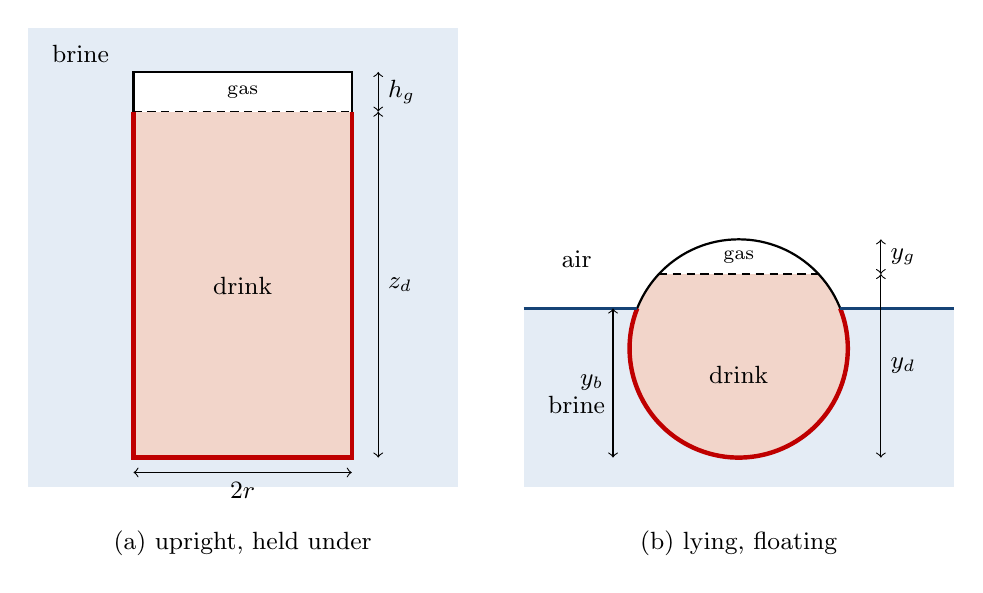
\begin{tikzpicture}[scale=0.42, every node/.style={font=\small}]
% (a) upright, held under
\fill[accentA!12] (-3.2,-0.9) rectangle (9.8,13.0);
\fill[white] (0,0) rectangle (6.6,11.66);
\fill[accentB!22] (0,0) rectangle (6.6,10.46);
\draw[thick] (0,0) rectangle (6.6,11.66);
\draw[densely dashed] (0,10.46) -- (6.6,10.46);
\draw[red!75!black, line width=1.6pt] (0,10.46) -- (0,0) -- (6.6,0) -- (6.6,10.46);
\node at (3.3,11.06) {\scriptsize gas};
\node at (3.3,5.2) {drink};
\node at (-1.6,12.2) {brine};
\draw[<->] (7.4,0) -- node[right] {$z_d$} (7.4,10.46);
\draw[<->] (7.4,10.46) -- node[right] {$h_g$} (7.4,11.66);
\draw[<->] (0,-0.45) -- node[below] {$2r$} (6.6,-0.45);
\node at (3.3,-2.6) {(a) upright, held under};
% (b) lying, floating
\begin{scope}[shift={(15,0)}]
\fill[accentA!12] (-3.2,-0.9) rectangle (9.8,4.51);
\fill[white] (3.3,3.3) circle (3.3);
\begin{scope}
\clip (3.3,3.3) circle (3.3);
\fill[accentB!22] (-0.1,-0.1) rectangle (6.7,5.55);
\end{scope}
\draw[thick] (3.3,3.3) circle (3.3);
\draw[densely dashed] (0.886,5.55) -- (5.714,5.55);
\draw[red!75!black, line width=1.6pt] (3.3,3.3) ++(158.49:3.3) arc[start angle=158.49, end angle=381.51, radius=3.3];
\draw[accentA!70!black, thick] (-3.2,4.51) -- (0.23,4.51);
\draw[accentA!70!black, thick] (6.37,4.51) -- (9.8,4.51);
\node at (3.3,6.05) {\scriptsize gas};
\node at (3.3,2.5) {drink};
\node at (-1.6,1.6) {brine};
\node at (-1.6,6.0) {air};
\draw[<->] (7.6,0) -- node[right] {$y_d$} (7.6,5.55);
\draw[<->] (7.6,5.55) -- node[right] {$y_g$} (7.6,6.6);
\draw[<->] (-0.5,0) -- node[left] {$y_b$} (-0.5,4.51);
\node at (3.3,-2.6) {(b) lying, floating};
\end{scope}
\end{tikzpicture}
\caption{Can~2 to scale, part-filled. (a) Upright and held under the brine: 1.2\,cm of headspace above
10.46\,cm of drink. (b) End-on, lying and floating in strong brine: a gas strip 1.05\,cm deep, drink
5.55\,cm deep, and the brine 4.51\,cm up the can. Heat passes only where the wall has drink inside and brine
outside (red).}
\label{fig:can}
\end{figure}

\subsection{Does the can float?}
\para{Derivation.} By Archimedes' principle, a floating body sinks until the liquid it displaces weighs as
much as it does. The can and drink weigh $(m_d + m_c)g$; a volume $V_{\mathrm{imm}}$ of brine of density
$\rho_b$ weighs $\rho_bgV_{\mathrm{imm}}$. So $V_{\mathrm{imm}} = (m_d + m_c)/\rho_b$, and if that is less than
the can's volume, the can floats. Upright, the immersed volume is $\pi r^2z_b$; lying, it is $\ell\,\Aseg(y_b)$:
\begin{equation}
z_b = \frac{m_d + m_c}{\rho_b\,\pi r^2},\qquad \Aseg(y_b) = \frac{m_d + m_c}{\rho_b\,\ell}. \label{eq:s9-float}
\end{equation}
For Can~2, 343\,g in all, in strong brine ($\rho_b = 1182$\,kg\,m$^{-3}$): $z_b = 8.48$\,cm upright,
$y_b = 4.51$\,cm lying. A part-filled can is lighter for its size, so it floats higher than a full one.

\para{Which way up?} Tilt a floating upright can by a small angle. The displaced brine shifts to the low
side and moves the centre of buoyancy B sideways, as if the can hung from a point M, the
\emph{metacentre}, a height $BM = I/V_{\mathrm{imm}}$ above B, where $I = \pi r^4/4$ is the second moment of
the can's cross-section at the brine surface. The can rights itself if M lies above its centre of mass.
Measuring from the bottom of the can, B is at $z_b/2$ and the centre of mass at about $z_d/2$, the middle of
the drink, so the height of M above the centre of mass is
\begin{equation}
GM = \frac{z_b}{2} + \frac{r^2}{4z_b} - \frac{z_d}{2} . \label{eq:s9-GM}
\end{equation}
For Can~2, $GM = 4.24 + 0.32 - 5.25 = -0.69$\,cm (the centre of mass at 5.25\,cm includes the can). The drink
sloshing inside, with a free surface of its own, lowers it further, by $(\rho_d/\rho_b)\,BM$, to $-0.97$\,cm.
$GM < 0$: an upright can floating in brine is unstable and \textbf{tips onto its side}. In fresh water it is
marginal ($+0.03$\,cm, and $-0.25$\,cm with the drink's free surface) and falls over too. A can that is not
held floats lying down, as in the rig.

\begin{worked}{Can 2 floating on its side}
The brine reaches $y_b = 4.51$\,cm up a can 6.6\,cm across, below the drink's 5.55\,cm, so the wall is wet on
both sides only below 4.51\,cm: $A_c = 200$\,cm$^2$, 64\,\% of the surface. The top centimetre of drink faces
the air in the box instead, which exchanges heat at only 5--10\,W\,m$^{-2}$K$^{-1}$, and is left out.
\end{worked}

\subsection{What the fill and the immersion do to the cooling}
Table~\ref{tab:fill} puts the areas into \eqref{eq:s8-G} and \eqref{eq:s8-fixed}, for a bath held at
$-18\dC$ and a drink starting at $28\dC$.

\begin{table}[ht]
\centering\small
\caption{Can~2 with a cola, cooled from $28\dC$ to $5\dC$ in a bath held at $-18\dC$.}
\label{tab:fill}
\begin{tabular}{@{}lcccc@{}}
\toprule
Can & $A_c$ (cm$^2$) & $G$ (W\,K$^{-1}$) & $\tau$ (s) & time to $5\dC$ (s)\\
\midrule
Whole surface passes heat (first estimate), upright & 310 & 5.00 & 266 & 185\\
Part-filled, upright, held under & 251 & 4.05 & 329 & 228\\
Part-filled, lying, held under & 240 & 4.64 & 287 & 199\\
Part-filled, lying, floating & 200 & 3.86 & 345 & 239\\
\bottomrule
\end{tabular}
\end{table}

Ignoring the headspace makes an upright can cool about 20\,\% too fast. Lying down loses wetted area but
gains stronger films, and ends only 8\,\% slower than the whole-surface estimate. Floating costs another
20\,\%: hold the can under.

\subsection{Room to freeze}
If the drink starts to freeze (Step~10), its ice takes more room than the water it came from:
$1/917 - 1/1000 = 9.05\times10^{-5}$\,m$^3$ per kg, about 0.09\,mL per gram of ice. The headspace takes up the
expansion by compressing its gas, whose pressure at constant temperature goes as $1/V$ (Boyle's law):
\begin{equation}
\frac{p}{p_0} = \frac{V_g}{V_g - \Delta V_{\mathrm{ice}}}, \qquad \Delta V_{\mathrm{ice}} = 9.05\times10^{-5}\,m_{\mathrm{ice}} . \label{eq:s9-pressure}
\end{equation}
240\,g of ice, Step~10's cola at $-5\dC$, needs 22\,mL. In a 41\,mL headspace that more than doubles the
pressure; in a real can's smaller headspace the can may bulge or burst.

% =====================================================================
\section{Step 10: the drink as a solution, an ethanol model (new)}\label{sec:s10}

\para{The idea.} A drink is water with things dissolved in it: sugar, carbon dioxide and, in a beer or a
cider, ethanol. They set two things: the drink's heat capacity $c_d$, which says how much heat must come
out, and its freezing point $\Tfd$, below which it starts to turn to slush. Dissolved molecules lower the
freezing point exactly as salt lowers the bath's (Step~6), but each counts once, since none splits into
ions.

\subsection{Composition from the label}
\para{Derivation.} Alcohol by volume, ABV, is the volume of ethanol per volume of drink. Per cubic metre of
drink, the ethanol's mass is $\rho_e\,\mathrm{ABV}$, with $\rho_e = 789.2$\,kg\,m$^{-3}$, and the drink's mass is
$\rho_d$; their ratio is the ethanol's mass fraction. Sugar and CO$_2$ are given as mass per volume, $s$ and
$c$ in g\,L$^{-1}$ (equal to kg\,m$^{-3}$); dividing by $\rho_d$ gives their mass fractions. Beer also holds
about 3.5\,\% of unfermented extract, $w_x$, mostly large molecules. The rest is water:
\begin{gather}
w_e = \frac{\rho_e\,\mathrm{ABV}}{\rho_d},\qquad w_{su} = \frac{s}{\rho_d},\qquad w_c = \frac{c}{\rho_d}, \label{eq:s10-fractions}\\
w_{wd} = 1 - w_e - w_{su} - w_c - w_x . \notag
\end{gather}
The molality of each solute is its moles per kilogram of the drink's water: its mass fraction over its molar
mass, divided by the water's mass fraction:
\begin{equation}
b_k = \frac{w_k}{M_k\,w_{wd}},\qquad k = e,\ su,\ c . \label{eq:s10-molality}
\end{equation}

\subsection{Where the drink starts to freeze}
\para{Derivation.} The derivation of \eqref{eq:s6-Kf} counted dissolved particles per kilogram of water,
whatever they were. Ethanol, sugar and CO$_2$ stay whole molecules in water, $i_v = 1$, so their molalities
simply add:
\begin{equation}
\boxed{\,\Tfd = -K_f\,(b_e + b_{su} + b_c)\,} \label{eq:s10-Tfd}
\end{equation}
The extract's molecules are large, so few per gram, and it is left out.

\begin{table}[ht]
\centering\small
\caption{Three drinks, from \eqref{eq:s10-fractions}--\eqref{eq:s10-Tfd} and \eqref{eq:s10-cd}.}
\label{tab:drinks}
\begin{tabular}{@{}lccc@{}}
\toprule
 & Cola & Beer, 5\,\% ABV & Hard seltzer, 5\,\% ABV\\
\midrule
Density $\rho_d$ (kg\,m$^{-3}$) & 1040 & 1008 & 993\\
Sugar; CO$_2$ (g\,L$^{-1}$) & 106 (sucrose); 6.5 & 0; 5.0 & 0; 6.0\\
Ethanol $w_e$; water $w_{wd}$ & 0; 0.892 & 0.039; 0.921 & 0.040; 0.954\\
$b_e$, $b_{su}$, $b_c$ (mol\,kg$^{-1}$) & 0, 0.334, 0.159 & 0.923, 0, 0.122 & 0.904, 0, 0.144\\
Freezing point $\Tfd$ & $-0.92\dC$ & $-1.94\dC$ & $-1.95\dC$\\
Specific heat $c_d$ (kJ\,kg$^{-1}$K$^{-1}$) & 3.95 & 4.14 & 4.24\\
\bottomrule
\end{tabular}
\end{table}

5\,\% of ethanol lowers the freezing point by 1.7\,K, more than the 10\,\% of sugar in a cola (0.6\,K): an
ethanol molecule has a seventh of the mass of a sucrose molecule, so per gram it counts seven times. Measured
freezing points of beers are close to $-2\dC$. Glucose--fructose syrup, whose molecules are half the mass of
sucrose's, counts twice per gram. The law is the dilute one; for spirits, such as 40\,\% ABV, use measured
freezing points.

\subsection{Freezing gradually: slush}
\para{Derivation.} Ice that forms in the drink is pure water; the ethanol, sugar and CO$_2$ stay in the
liquid, which gets stronger as it loses water. If a share $\psi$ of the drink's water has frozen, every
molality is $1/(1 - \psi)$ times its starting value, and by \eqref{eq:s10-Tfd} so is the freezing-point drop.
The liquid that is left is in equilibrium with the ice when
\begin{equation}
T_d = \frac{\Tfd}{1 - \psi}\qquad\Longleftrightarrow\qquad \psi(T_d) = 1 - \frac{\Tfd}{T_d}\quad (T_d < \Tfd). \label{eq:s10-psi}
\end{equation}
Below $\Tfd$ the drink is a slush whose ice grows as it cools: half its water frozen at $2\Tfd$, three
quarters at $4\Tfd$.

Freezing releases latent heat, which the bath must take away. The drink's energy, measured as in Step~8,
gains a latent term for its ice; neglecting the small difference between the heat capacities of its ice and
its water,
\begin{equation}
U_D = C_d\,(T_d - T_{\mathrm{ref}}) - L_f\,m_{wd}\,\psi(T_d), \label{eq:s10-UD}
\end{equation}
with $m_{wd} = w_{wd}m_d$ the water in the drink. Differentiating with respect to $T_d$, with
$\dd\psi/\dd T_d = \Tfd/T_d^2$ from \eqref{eq:s10-psi} (negative, since $\Tfd < 0$: more ice as it cools),
gives the heat that cools the drink by one kelvin, its effective heat capacity:
\begin{equation}
\boxed{\begin{aligned}
\Cdeff(T_d) &= C_d + \frac{L_f\,m_{wd}\,|\Tfd|}{T_d^2} &&(T_d < \Tfd),\\
\Cdeff(T_d) &= C_d &&(T_d \ge \Tfd)
\end{aligned}} \label{eq:s10-Ceff}
\end{equation}
and the drink's equation \eqref{eq:s8-drink} becomes $\Cdeff(T_d)\,\dot T_d = -\dot Q_d$.

\begin{worked}{a beer and a cola left in}
Beer: 304\,g of water, $\Tfd = -1.94\dC$. Just below $\Tfd$, $\Cdeff$ jumps from 1.38\,kJ\,K$^{-1}$ to
53\,kJ\,K$^{-1}$, forty times larger, so the drink lingers near $-2\dC$ while it freezes. At $-5\dC$ it is
61\,\% frozen (186\,g of ice, 17\,mL of expansion); at $-17\dC$, 89\,\%. A cola, $\Tfd = -0.92\dC$ with 294\,g of
water, is 82\,\% frozen at $-5\dC$ (240\,g of ice, 22\,mL). Ethanol keeps a beer liquid a kelvin lower, but a
drink left in a $-20\dC$ bath ends mostly ice either way.
\end{worked}

\subsection{The drink's heat capacity}
\para{Derivation.} A solution's heat capacity is a sum over what it contains, each part weighted by its mass
fraction and counted with its \emph{partial} specific heat: what a kilogram of it adds to the solution,
which is not its heat capacity as a pure substance:
\begin{equation}
c_d = w_{wd}\,c_w + w_e\,\bar c_e + w_{su}\,\bar c_{su} + w_x\,\bar c_x . \label{eq:s10-cd}
\end{equation}
In dilute solution ethanol adds about 5.4\,kJ\,kg$^{-1}$K$^{-1}$ (0.25\,kJ\,mol$^{-1}$K$^{-1}$), more than twice
pure ethanol's 2.44 and more than water's: water molecules order themselves round the ethanol's ethyl group,
and that order melts as the solution warms, which takes heat. Sucrose adds about 1.9\,kJ\,kg$^{-1}$K$^{-1}$ and
beer's extract about 1.5; the CO$_2$ is too little to matter. So a little ethanol \emph{raises} $c_d$ slightly
above water's, while sugar lowers it: the values in Table~\ref{tab:drinks}. A mass-weighted average with
pure ethanol's 2.44 would wrongly put a beer below water.

These are estimates, good to a few per cent. A drink's own value is easily measured by mixing: pour a mass
$m_1$ of drink at $T_1$ into a mass $m_2$ of water at $T_2$ in an insulated cup and read the final
temperature $T_3$. The heat the drink loses is the heat the water gains, so
$c_d = m_2c_w(T_3 - T_2)/[m_1(T_1 - T_3)]$.

\subsection{Convection inside the can}
At 5\,\% ethanol the drink is about 15\,\% more viscous than water and slightly less conductive; through the
quarter powers of Step~8 these change $h_i$ by a few per cent. More important near the end of a run: water is
densest at $4\dC$, and as the drink at the wall approaches that temperature it stops getting denser, so the
free convection that mixes it weakens. Dissolved sugar and CO$_2$ move that point lower. The usual target,
$5\dC$, is just above it.

\subsection{Supercooling}
A still drink in a smooth can often cools several kelvin below $\Tfd$ before any ice appears, then freezes
part of the way within seconds, its latent heat warming it back onto the curve \eqref{eq:s10-psi}. The model
assumes ice appears at $\Tfd$.

\subsection{What ethanol changes}
In the coupled model of Step~11 a beer takes 3\,\% longer than a cola to reach $5\dC$
(the worked example of Step~11), because its $c_d$ is larger. Ethanol matters little for the cooling time; it matters
for what happens after, by keeping the drink liquid a kelvin lower.

\subsection{Ethanol in the bath instead of salt}
The same law describes ice with ethanol in place of salt, with $i_v = 1$ and $M_e = 0.04607$\,kg\,mol$^{-1}$:
per unit of the mass ratio $m_s/W$, ethanol lowers the freezing point by $K_f/M_e = 40.4$\,K against salt's
63.7\,K, so in dilute solution salt is the stronger by weight. Two things differ more. Ethanol mixes with
water in any proportion, so there is no saturation and no eutectic plateau within reach: such a bath has no
thermostat, and warms as its ice melts. And mixing ethanol with water releases heat, where dissolving salt
absorbs it. This document does not model an ethanol bath further.

% =====================================================================
\section{Step 11: fully unified time-dependent model, with the can}\label{sec:s11}

\para{The idea.} Put the pieces together: the bath's energy balance (Step~5) with the drink's heat in it,
the freezing point (Step~6) tying the bath temperature to its salt and water, the dissolution rate
(Step~7), and the drink's equation (Steps~8 and~10). Then solve for the rates.

\para{Shortcuts} (the first edition's, and the can's):
\begin{align}
W &= M_w - m_i = m_w, \label{eq:s11-W}\\
\Ceff &= m_ic_i + Wc_w, \label{eq:s11-Ceff}\\
\alpha &= \frac{i_vK_f}{\MN},\qquad \beta = \frac{\Hsol}{\MN},\qquad H = \frac{kA}{d},\qquad G = \hov A_c . \label{eq:s11-short}
\end{align}
$\alpha$ is in kelvin per unit of the mass ratio $m_s/W$, and $\beta$ in J\,kg$^{-1}$.

\para{Derivation.} The bath now receives heat from the room and from the drink. Call their sum
\begin{equation}
\dot Q_{\mathrm{in}} = H(\Troom - T) + G(T_d - T); \label{eq:s11-Qin}
\end{equation}
it replaces the left side of \eqref{eq:s5-balance}, whose right side is unchanged. The freezing point is
\eqref{eq:s6-T}:
\begin{align}
\dot Q_{\mathrm{in}} &= \Ceff\,\dot T - L_f\,\dot m_i + \beta\,\dot m_s, \label{eq:s11-balance}\\
T &= -\alpha\,\frac{m_s}{W}. \label{eq:s11-T}
\end{align}
Differentiate \eqref{eq:s11-T} with the quotient rule, using $\dot W = -\dot m_i$ from \eqref{eq:s11-W}:
\begin{align}
\dot T &= -\alpha\,\frac{\dd}{\dd t}\Big(\frac{m_s}{W}\Big) \label{eq:s11-Tdot1}\\
&= -\alpha\,\frac{\dot m_sW - m_s\dot W}{W^2} \label{eq:s11-Tdot2}\\
&= -\alpha\Big(\frac{\dot m_s}{W} + \frac{m_s\,\dot m_i}{W^2}\Big). \label{eq:s11-Tdot}
\end{align}
Dissolving salt cools the bath (the first term); melting ice warms it, since $\dot m_i < 0$ (the second).
Substituting \eqref{eq:s11-Tdot} into \eqref{eq:s11-balance}, then collecting the terms in $\dot m_s$ and in
$\dot m_i$:
\begin{align}
\dot Q_{\mathrm{in}} &= -\alpha\Ceff\Big(\frac{\dot m_s}{W} + \frac{m_s\,\dot m_i}{W^2}\Big) - L_f\,\dot m_i + \beta\,\dot m_s \label{eq:s11-sub}\\
&= \Big(\beta - \frac{\alpha\Ceff}{W}\Big)\dot m_s - \Big(L_f + \frac{\alpha\Ceff m_s}{W^2}\Big)\dot m_i . \label{eq:s11-collect}
\end{align}
Solving for the ice, and writing $\dot Q_{\mathrm{in}}$ out again:
\begin{equation}
\boxed{\,\dot m_i = \frac{\Big(\beta - \dfrac{\alpha\Ceff}{W}\Big)\dot m_s - H(\Troom - T) - G(T_d - T)}{L_f + \dfrac{\alpha\Ceff m_s}{W^2}}\,} \label{eq:s11-mi}
\end{equation}

\para{What the terms mean.} The denominator is the heat it takes to melt a kilogram of ice \emph{in this
bath}: $L_f$, plus the heat that warms the whole bath, because the meltwater dilutes the brine and raises its
freezing point. In the numerator, heat from the room and from the drink melts ice. Dissolving salt melts ice
too, through the bracket, which is negative in practice: the salt lowers the freezing point, the bath must
cool to follow it, and the heat for that cooling comes from melting ice. This is how a salted ice bath cools
itself.

\begin{worked}{the rig bath as the can goes in}
After 15 minutes with no stirrer (the run below): $m_s = 0.633$\,kg and $T = -16.8\dC$, so
$W = \alpha m_s/|T| = 2.40$\,kg, $m_i = 3.20$\,kg and $\Ceff = 16.8$\,kJ\,K$^{-1}$. The denominator is
$333\,500 + 116\,800 = 450\,300$\,J\,kg$^{-1}$, 35\,\% more than $L_f$. The bracket is
$66\,700 - 443\,800 = -377\,100$\,J\,kg$^{-1}$: each kilogram of salt that dissolves melts
$377\,100/450\,300 = 0.84$\,kg of ice.
\end{worked}

\para{The drink.} From Steps~8 and~10:
\begin{equation}
\Cdeff(T_d)\,\dot T_d = -G\,(T_d - T). \label{eq:s11-drink}
\end{equation}

\para{The full reduced system.}
\begin{equation}
\boxed{
\begin{aligned}
\dot m_s &= k_mA_{s,0}\Big(\frac{m_{s,0} - m_s}{m_{s,0}}\Big)^{2/3}\Big[\Csat(T) - \frac{\rho_wm_s}{W}\Big],\\
\dot m_i &= \frac{\big(\beta - \frac{\alpha\Ceff}{W}\big)\dot m_s - H(\Troom - T) - G(T_d - T)}{L_f + \frac{\alpha\Ceff m_s}{W^2}},\\
\dot T_d &= -\frac{G\,(T_d - T)}{\Cdeff(T_d)},\\
T &= -\alpha\,\frac{m_s}{W},\qquad W = M_w - m_i,\qquad \Ceff = m_ic_i + Wc_w .
\end{aligned}}
\label{eq:s11-system}
\end{equation}
Three state variables, $m_s$, $m_i$ and $T_d$, move by the three rate equations; the bath temperature follows
from the last line. Start with $m_i(0)$ and $m_s(0)$ consistent with \eqref{eq:s11-T}, and $T_d(0)$ the
drink's starting temperature; before the can goes in, set $G = 0$. This \emph{ice--brine equilibrium branch}
stops applying when the ice runs out, when the brine saturates (then $\dot m_s = 0$ and the bath sits near
\eqref{eq:s6-TE}), or when the bath is far from phase equilibrium.

\para{Alternative single implicit equation.} Eliminating $T$ from the heat balance with \eqref{eq:s11-T},
without solving for $\dot m_i$:
\begin{multline}
H\Big(\Troom + \frac{\alpha m_s}{W}\Big) + G\Big(T_d + \frac{\alpha m_s}{W}\Big)\\
= -\alpha\Ceff\Big(\frac{\dot m_s}{W} + \frac{m_s\,\dot m_i}{W^2}\Big) - L_f\,\dot m_i + \beta\,\dot m_s . \label{eq:s11-implicit}
\end{multline}
It is equivalent to \eqref{eq:s11-mi} paired with \eqref{eq:s11-T}.

\begin{worked}{the rig with Can 2, solved}
\eqref{eq:s11-system} integrated numerically with the rig's numbers: a box of 0.46\,W\,K$^{-1}$ and a room at
$28\dC$; the $4\dC$ water first melts 80\,g of ice so that the bath starts at $0\dC$; grains 0.5\,mm across,
$A_{s,0} = 5.5$\,m$^2$; $\Csat = 357$\,kg\,m$^{-3}$ held constant; the can goes in at $28\dC$ after 15 minutes.

\smallskip
{\small\centering
\begin{tabular}{@{}lccc@{}}
\toprule
 & & \multicolumn{2}{c}{time to $5\dC$ (s)}\\
\cmidrule(l){3-4}
Can & $G$ (W\,K$^{-1}$) & $k_m = 10^{-6}$ & $k_m = 10^{-5}$\\
\midrule
Whole surface passes heat, upright & 5.00 & 192 & 165\\
Part-filled, upright, held under & 4.05 & 235 & 202\\
Part-filled, lying, held under & 4.64 & 207 & 176\\
Part-filled, lying, floating & 3.86 & 246 & 213\\
As above, with a beer & 4.64 & 213 & 183\\
\midrule
Bath when the can goes in & & $-16.8\dC$ & $-22.4\dC$\\
Salt dissolved by then & & 0.63\,kg & 0.93\,kg\\
\bottomrule
\end{tabular}\par}

\smallskip
$k_m$ is in m\,s$^{-1}$. With still brine ($k_m = 10^{-6}$) the salt dissolves slowly and the bath is only at $-16.8\dC$ after 15
minutes; with brine moving past the grains ($10^{-5}$) it has nearly reached the model's floor, $-22.7\dC$.
A drink left in for two hours ends at $-19.2\dC$: a cola 95\,\% frozen, a beer 90\,\%.
\end{worked}

% =====================================================================
\section{Step 12: time-independent equilibrium, with the can}\label{sec:s12}

\para{The idea.} There are two different things ``time-independent'' can mean: energy accounting between
two moments, and a true steady state that nothing changes any more. They are not interchangeable.

\subsection{Insulated equilibrium}
\para{Derivation.} With no heat in, \eqref{eq:s1-dU} says the energy at the end equals the energy at the
start, $U_f = U_0$. Measure energies from ice and liquid water at $T_0 = 0\dC$, with the first edition's
reference: liquid water holds $L_f$ per kilogram more than ice. Between start and end, ice and water warm
or cool to $T_f$ (sensible heat), $m_{i,0} - m_{i,f}$ of ice melts (latent energy gained) and
$m_{s,f} - m_{s,d,0}$ of salt dissolves (heat of solution absorbed); their sum is zero:
\begin{equation}
\boxed{\,0 = (m_{i,f}c_i + m_{w,f}c_w)\,T_f - L_f\,(m_{i,f} - m_{i,0}) + \beta\,(m_{s,f} - m_{s,d,0})\,} \label{eq:s12-insulated}
\end{equation}
With ice and brine together at the end, the mass balance and the freezing point close it:
\begin{align}
m_{w,f} &= M_w - m_{i,f}, \label{eq:s12-mw}\\
T_f &= -\alpha\,\frac{m_{s,f}}{M_w - m_{i,f}} . \label{eq:s12-Tf}
\end{align}
If solid salt remains, the brine is saturated, which is a third condition:
\begin{equation}
C_f = \Csat(T_f); \label{eq:s12-sat}
\end{equation}
if all the salt has dissolved, $m_{s,f} = S_0$ instead. These are alternative regimes, not simultaneous
conditions: try one, and check that its answer is consistent.

\para{With the can, and other starting temperatures (new).} The drink cools from $T_{d,0}$ to $T_f$; if
$T_f < \Tfd$ part of its water freezes, by \eqref{eq:s10-psi}, giving up latent heat. Water starting at
$T_{w,0}$ and salt at $T_{s,0}$ bring their own sensible heat, measured from $0\dC$, on the starting side; the
salt that is still solid at the end is counted at $T_f$ (Step~5's correction). With the ice starting at
$0\dC$:
\begin{multline}
0 = \big[m_{i,f}c_i + m_{w,f}c_w + (S_0 - m_{s,f})\,c_s\big]\,T_f - L_f\,(m_{i,f} - m_{i,0})\\
+ \beta\,(m_{s,f} - m_{s,d,0}) + C_d\,(T_f - T_{d,0}) - L_f\,m_{wd}\,\psi(T_f)\\
- m_{w,0}c_wT_{w,0} - S_0c_sT_{s,0} . \label{eq:s12-can}
\end{multline}

\begin{worked}{the rig and Can 2, left until everything settles}
Rig numbers, with the drink at $28\dC$; ``measured diagram'' means the freezing curve, solubility and eutectic
of the B8 report's model (\texttt{b8\_sim.py}) instead of \eqref{eq:s12-Tf}--\eqref{eq:s12-sat}.

\smallskip
{\small\centering
\begin{tabular}{@{}lcccc@{}}
\toprule
 & $T_f$ & ice left & solid salt left & drink frozen\\
\midrule
Bath alone, dilute law & $-22.7\dC$ & 2.85\,kg & 19\,g (saturated) & ---\\
Bath alone, measured diagram & $-21.2\dC$ & 2.93\,kg & 193\,g & ---\\
With a cola, dilute law & $-20.3\dC$ & 2.46\,kg & 0 & 95\,\%\\
With a cola, measured diagram & $-21.2\dC$ & 2.42\,kg & 40\,g & 96\,\%\\
With a beer, dilute law & $-20.3\dC$ & 2.46\,kg & 0 & 90\,\%\\
With a beer, measured diagram & $-21.2\dC$ & 2.42\,kg & 40\,g & 91\,\%\\
\bottomrule
\end{tabular}\par}

\smallskip
The drink gives the bath about 160\,kJ, cooling from $28\dC$ and freezing, which melts 0.4--0.5\,kg of ice.
With the dilute law that dissolves the last of the salt and leaves the bath at $-20.3\dC$; with the measured
diagram the bath stays on its eutectic plateau at $-21.2\dC$ and uses 150\,g of its spare salt. (A beer and a
cola give almost the same heat: the beer's larger heat capacity is offset by its smaller frozen share.) Either
way a can left until everything settles is mostly ice: take it out at $5\dC$.
\end{worked}

\subsection{Integrated heat leakage over a finite interval}
\para{Derivation.} Integrating the bath balance \eqref{eq:s11-balance} from $0$ to $t_f$, for constant
$c_i$, $c_w$, $L_f$ and $\beta$, the latent and dissolution terms integrate exactly, but the sensible term does
not, because $\Ceff$ changes as ice melts:
\begin{multline}
\int_0^{t_f}\big\{H[\Troom - T(t)] + G[T_d(t) - T(t)]\big\}\,\dd t\\
= \int_0^{t_f}\Ceff(t)\,\dot T(t)\,\dd t - L_f(m_{i,f} - m_{i,0}) + \beta(m_{s,f} - m_{s,d,0}) . \label{eq:s12-integral}
\end{multline}
The first edition's endpoint formula,
\begin{multline}
\int_0^{t_f} H[\Troom - T(t)]\,\dd t\\
\overset{\text{earlier approximation}}{\approx} C_fT_f - C_0T_0 - L_f(m_{i,f} - m_{i,0}) + \beta(m_{s,f} - m_{s,d,0}), \label{eq:s12-earlier}
\end{multline}
is not generally valid when $\Ceff$ varies.

\begin{correction}
\textbf{Correction} (first edition). Integrating by parts,
\begin{equation}
\int_0^{t_f}\Ceff\,\dot T\,\dd t = \big[\Ceff T\big]_0^{t_f} - \int_0^{t_f} T\,\dot C_{\mathrm{eff}}\,\dd t,\qquad
\dot C_{\mathrm{eff}} = (c_i - c_w)\,\dot m_i , \label{eq:s12-parts}
\end{equation}
so \eqref{eq:s12-integral}, not the endpoint replacement \eqref{eq:s12-earlier}, follows the rate equation
literally.
\end{correction}
The drink's part, by contrast, integrates exactly: from \eqref{eq:s11-drink}, $G(T_d - T) = -\Cdeff\dot T_d$,
so the heat it gives the bath between two moments is $C_d(T_{d,0} - T_d)$, plus $L_fm_{wd}\psi$ if it has
started to freeze. Its heat capacity, unlike the bath's, does not change.

\subsection{True steady state with heat leakage}
\para{Derivation.} In a steady state nothing changes: $\dot T = \dot m_i = \dot m_s = \dot T_d = 0$. Then
\eqref{eq:s11-drink} gives $G(T_d - T) = 0$, and \eqref{eq:s11-balance} gives $H(\Troom - T) = 0$:
\begin{align}
H(\Troom - T_{\mathrm{eq}}) &= 0,\qquad G(T_{d,\mathrm{eq}} - T_{\mathrm{eq}}) = 0, \label{eq:s12-steady}\\
T_{\mathrm{eq}} &= T_{d,\mathrm{eq}} = \Troom\qquad (H > 0,\ G > 0). \label{eq:s12-Teq}
\end{align}
Above $0\dC$ no ice can be in equilibrium, so the true steady state comes only after all the ice has melted;
it cannot be found by imposing the ice--brine freezing condition on a warm room.

% =====================================================================
\section{A thermodynamically more consistent refinement}\label{sec:refine}

\para{The idea.} The model so far treats $L_f$ as a constant while giving ice and water different specific
heats, $c_i \ne c_w$. That is inconsistent away from $0\dC$. A consistent model starts from an energy that is a
function of the state, and differentiates it.

\para{Derivation.} Choose $T_{\mathrm{ref}} = 0\dC$; give ice zero energy there, and liquid water $L_f$.
In a first ideal-mixture approximation, the bath's energy is
\begin{equation}
U_{\mathrm{approx}} = m_ic_i\,(T - T_{\mathrm{ref}}) + m_w\big[L_f + c_w(T - T_{\mathrm{ref}})\big] + \beta\,m_s . \label{eq:refine-U}
\end{equation}
Differentiating with the product rule, and using $\dot m_w = -\dot m_i$:
\begin{equation}
\dot U_{\mathrm{approx}} = (m_ic_i + m_wc_w)\,\dot T + \big[(c_i - c_w)(T - T_{\mathrm{ref}}) - L_f\big]\,\dot m_i + \beta\,\dot m_s . \label{eq:refine-Udot}
\end{equation}
Setting this equal to the heat flowing in, now including the drink's:
\begin{multline}
H(\Troom - T) + G(T_d - T)\\
= (m_ic_i + m_wc_w)\,\dot T - \big[L_f + (c_w - c_i)(T - T_{\mathrm{ref}})\big]\,\dot m_i + \beta\,\dot m_s . \label{eq:refine-balance}
\end{multline}
At $T = T_{\mathrm{ref}}$ this is the simpler balance \eqref{eq:s11-balance}. Elsewhere the heat to melt a
kilogram of ice is $L_f + (c_w - c_i)(T - T_{\mathrm{ref}})$, smaller below zero (Kirchhoff's law): at
$-15\dC$, $333\,500 - 2080\times15 = 302\,300$\,J\,kg$^{-1}$, 9\,\% less. A more precise model would add the
brine's salt-dependent heat capacity and density, non-ideal mixing, the measured NaCl liquidus, and the
hydrated solid phase where it forms.

\subsection{Consistent integrated energy at any starting and final temperature}
\para{Derivation.} With an energy function, the integrated balance is exact: the heat let in equals the
change of energy. The drink's heat flows inside the system and cancels \eqref{eq:s1-sum}, so for bath and
drink together, with $U_D$ from \eqref{eq:s10-UD} and the undissolved salt's sensible heat included:
\begin{equation}
\boxed{\,\int_0^{t_f} H(\Troom - T)\,\dd t = \big[U_{\mathrm{approx}} + (S_0 - m_s)\,c_s(T - T_{\mathrm{ref}}) + U_D\big]_0^{t_f}\,} \label{eq:refine-integral}
\end{equation}
Written out, with the bath at $T_0$ and the drink at $T_{d,0}$ at the start:
\begin{multline}
\int_0^{t_f} H(\Troom - T)\,\dd t = m_{i,f}c_i(T_f - T_{\mathrm{ref}}) - m_{i,0}c_i(T_0 - T_{\mathrm{ref}})\\
+ m_{w,f}\big[L_f + c_w(T_f - T_{\mathrm{ref}})\big] - m_{w,0}\big[L_f + c_w(T_0 - T_{\mathrm{ref}})\big]\\
+ \beta\,(m_{s,f} - m_{s,d,0}) + (S_0 - m_{s,f})\,c_s(T_f - T_{\mathrm{ref}}) - S_0\,c_s(T_0 - T_{\mathrm{ref}})\\
+ C_d\,(T_{d,f} - T_{d,0}) - L_f\,m_{wd}\,\psi(T_{d,f}) . \label{eq:refine-expanded}
\end{multline}
This is the preferred endpoint equation for the idealised, constant-coefficient model. For a perfectly
insulated box, set the left side to zero. For a real box over a finite time, the left side depends on the
unknown history of $T$ and cannot be found from the endpoints alone.

% =====================================================================
\section{Model limits and practical next steps}\label{sec:limits}

\begin{enumerate}
\item \textbf{Initial temperature consistency.} The condition $T = -\alpha m_s/m_w$ cannot hold for pure ice and
  fresh water above $0\dC$, or for brine that has not reached its ice yet. The first moments of a run are out
  of equilibrium; start the model once ice and brine have met, or add a non-equilibrium start.
\item \textbf{Salt concentration.} The $i_vK_fb$ law suits dilute brine only (Step~6). Use the measured NaCl
  freezing curve and eutectic for the bath's working range.
\item \textbf{Dissolution kinetics.} Rates depend on grain size, crust, and whether brine flows through the
  ice. Measure or fit $k_m$ and $A_{s,0}$.
\item \textbf{The box.} $H = kA/d$ assumes flat, steady walls with faces at room and bath temperature.
  Calibrating $H$ with a box test is more reliable than computing it.
\item \textbf{Switching of phases.} Enforce $m_i \ge 0$, $0 \le m_s \le S_0$ and saturation. Ice--brine
  equilibrium, saturated brine with salt, all-liquid and eutectic regimes each need their own closure.
\item \textbf{The can is not a cylinder.} Its neck and domed base change the volumes and areas of Step~9 by
  several per cent: measure the brimful volume and the headspace.
\item \textbf{Hold the can under.} A free can floats lying down with a third of its wall out of the brine,
  and cools 20\,\% more slowly (Table~\ref{tab:fill}).
\item \textbf{The bath next to the can.} With no stirrer the brine near the can warms first, and the ice there
  melts first; one bath temperature overstates the cooling. The B8 report splits the bath into rings to
  follow this.
\item \textbf{The drink.} It stratifies slowly; its free convection weakens near $4\dC$; it may supercool,
  then partly freeze at once; and a frozen drink may burst its can.
\item \textbf{Drink data.} The freezing points and heat capacities of Step~10 come from dilute laws and
  approximate partial heat capacities. Measure $\Tfd$ from a slow cooling curve (the plateau where ice
  appears) and $c_d$ by mixing.
\item \textbf{Validation.} Compare predicted temperature--time curves and end states with experiments at
  several salt-to-water ratios, starting masses and temperatures, and insulation thicknesses; and, for the
  can, with probes in the drink and in the brine next to it, for full and part-filled cans, upright and
  lying, held and floating, and for drinks with and without ethanol.
\end{enumerate}

% =====================================================================
\section{Quick index of principal equations}\label{sec:index}

First law with the can: \eqref{eq:s1-bath}--\eqref{eq:s1-sum}. Conduction through the box: \eqref{eq:s2-Q},
with films \eqref{eq:s2-films}. Ice and water conservation: \eqref{eq:s4-mw}. Latent energy:
\eqref{eq:s3-balance}. NaCl energy: \eqref{eq:s5-Qsol} and \eqref{eq:s5-balance}. Freezing depression:
\eqref{eq:s6-Tf}--\eqref{eq:s6-T}; the model's floor \eqref{eq:s6-TE}. Dissolution kinetics:
\eqref{eq:s7-rate}--\eqref{eq:s7-boxed}. The drink and its can: \eqref{eq:s8-drink}, \eqref{eq:s8-G},
\eqref{eq:s8-fixed}. A part-filled can: \eqref{eq:s9-upright}--\eqref{eq:s9-lying}; floating
\eqref{eq:s9-float}, \eqref{eq:s9-GM}; room to freeze \eqref{eq:s9-pressure}. The ethanol model:
\eqref{eq:s10-fractions}--\eqref{eq:s10-cd}. Dynamic derivatives: \eqref{eq:s11-Tdot} and \eqref{eq:s11-mi};
the full system \eqref{eq:s11-system}. Insulated equilibrium: \eqref{eq:s12-insulated}--\eqref{eq:s12-can}.
Finite-time energy: \eqref{eq:s12-integral}. True steady state: \eqref{eq:s12-Teq}. Thermodynamically
consistent update: \eqref{eq:refine-balance}--\eqref{eq:refine-expanded}.

\end{document}
